\part{System Infrastructure}
\newpage
\chapter{Mechanical Infrastructure}

\section{Introduction}
The objective of our project was to design and build a prototype robot equipped with a mecanum
wheel system and a camera fixation. This robot is intended to showcase advanced maneuverability
and vision capabilities, making it suitable for various applications including surveillance,
inspection, and autonomous navigation. The design and construction were carried out using
SolidWorks, a powerful CAD software, to ensure precision and
functionality.

\section{Design Process} 
\subsection{Conceptualization} 
The initial phase involved brainstorming and conceptualizing the robot's design. We focused on
creating a compact and robust chassis that could support the mecanum wheels and the camera
system. The key requirements identified were:
\begin{itemize}
	\item Enhanced mobility with omnidirectional movement.
	\item Stable and secure mounting for the camera.
	\item Durability and ease of maintenance.
\end{itemize}


\subsection{CAD Modeling Using SolidWorks}
Using SolidWorks, we created detailed 3D models of the robot components. This phase included
iterative design and simulation to optimize the robot's performance and ensure all parts fit together
seamlessly. The major components designed were:
\begin{itemize}
	\item Robot chassis.
	\item Mecanum wheels.
	\item Camera fixation mount.
\end{itemize}

\newpage

\section{Robot Chassis}
\subsection{Material Selection}
The chassis was designed to be lightweight yet sturdy. We selected hard wood for the following
reasons:
\begin{itemize}
	\item High strength-to-weight ratio.
	\item Ease of machining and fabrication.
	\item Cost.
\end{itemize}


\subsection{Chassis Design}
The chassis was designed as a Circular frame with mounting points for the wheels and the camera
system. The key features include:
\begin{itemize}
	\item Central platform for mounting the control electronics and power supply.
	\item Four corner brackets for attaching the mecanum wheels.
	\item Slots and holes for cable management.
\end{itemize}


\subsection{Fabrication}
The chassis components were fabricated using CNC machining to ensure precision. The parts were
then assembled using screws and bolts, providing a robust structure capable of withstanding
operational stresses.

\section{Mecanum Wheels}

\subsection{Introduction to Mecanum Wheels}
Mecanum wheels are a type of omnidirectional wheel that allows a vehicle to move in any direction,
including sideways, without changing its orientation. This capability is achieved through the unique
design of the wheels, which feature rollers set at a 45-degree angle to the wheel’s axis.

\newpage
\subsection{Design and Selection}
For our robot, we selected commercially available mecanum wheels compatible with our chassis
dimensions and load requirements. The key specifications considered were:
\begin{itemize}
	\item Wheel diameter and width.
	\item Roller material and configuration.
	\item  Load-bearing capacity.
\end{itemize}

\subsection{Integration}
The mecanum wheels were mounted on the chassis using custom-designed brackets. Each wheel
was connected to an individual motor, enabling precise control of movement. The motors were
chosen based on torque and speed requirements to ensure smooth and responsive operation.

\section{Camera Fixation}
\subsection{Requirements}
The camera fixation system needed to provide a stable and adjustable platform for mounting the
camera. The key requirements were:
\begin{itemize}
	\item Stability to avoid vibrations and ensure clear imaging.
	\item Adjustability to change the camera angle and orientation.
	\item Compatibility with various camera models.
\end{itemize}


\subsection{Design}
The camera fixation system was designed as a gimbal-like structure, allowing for both pan and tilt
adjustments. The design features included:
\begin{itemize}
	\item A base plate mounted on the chassis.
	\item Adjustable arms for changing the camera’s position.
	\item Locking mechanisms to secure the camera in place.
\end{itemize}

\newpage
\subsection{Fabrication and Assembly}
The camera fixation components were fabricated using a combination of 3D printing and CNC
machining. This approach allowed for rapid prototyping and testing. The parts were assembled and
tested to ensure stability and ease of adjustment.
\section{Testing and Validation}
\subsection{Mobility Testing}
The robot was tested for its mobility in various environments. The mecanum wheels provided
excellent maneuverability, allowing the robot to navigate tight spaces and perform complex
movements. The tests included:
\begin{itemize}
	\item Forward and backward movement.
	\item Sideways movement.
	\item Diagonal movement.
	\item Rotational movement.
\end{itemize}


\subsection{Camera Stability Testing}
The camera fixation system was tested for stability and adjustability. The tests involved:
\begin{itemize}
	\item Evaluating the ease of adjusting the camera angle.
	\item Assessing the stability of the camera during movement.
	\item Ensuring the camera remained secure in its fixed position.
\end{itemize}


\subsection{Durability Testing}
The overall durability of the robot was tested by subjecting it to various stress conditions. These
included:
\begin{itemize}
	\item Impact tests to assess the chassis’ strength.
	\item Prolonged operation to test the endurance of the motors and wheels.
	\item Environmental tests to evaluate performance under different conditions.
\end{itemize}

\newpage

\section{Output} % + state which of the listed specs were fulfilled here

\begin{figure}[h!]
	\centering
	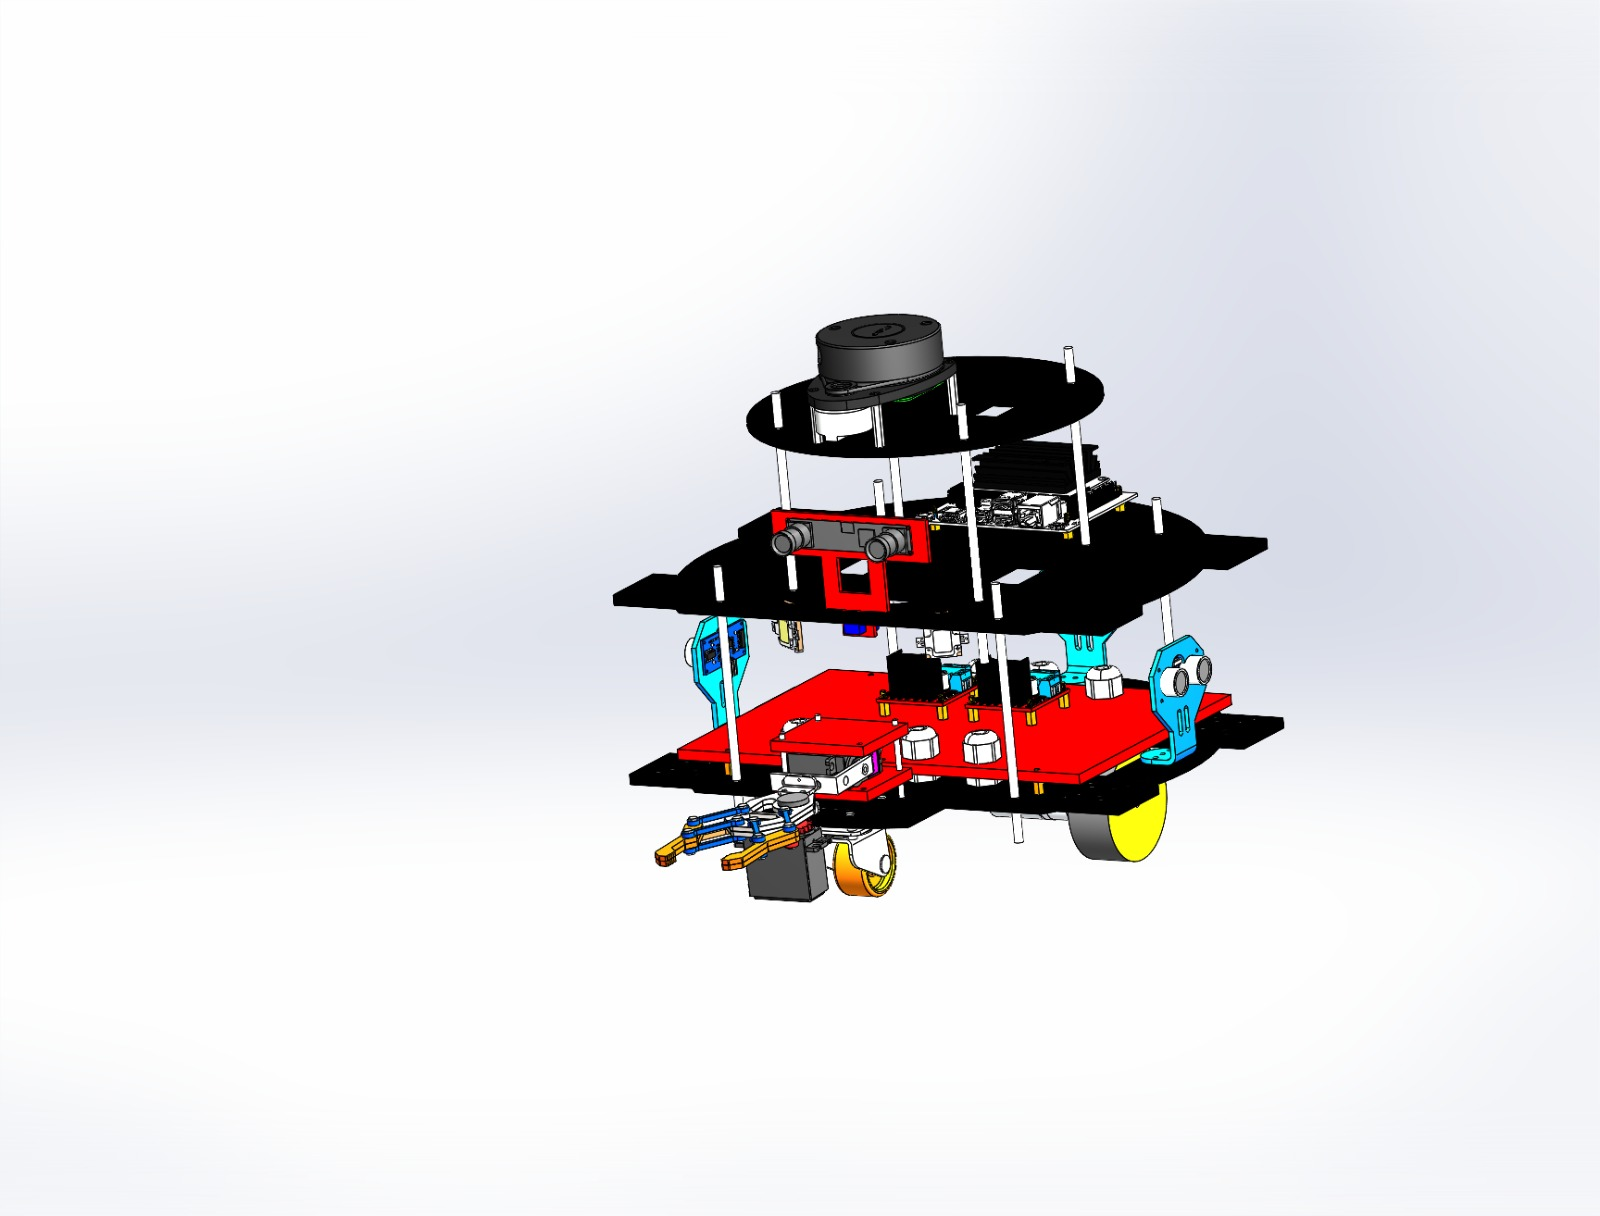
\includegraphics[scale=0.23]{./Figures/Mech/full.jpeg}
	\caption{Final Design -- Full view}
	\label{fig:mech1}
\end{figure}

\begin{figure}[h!]
	\centering
	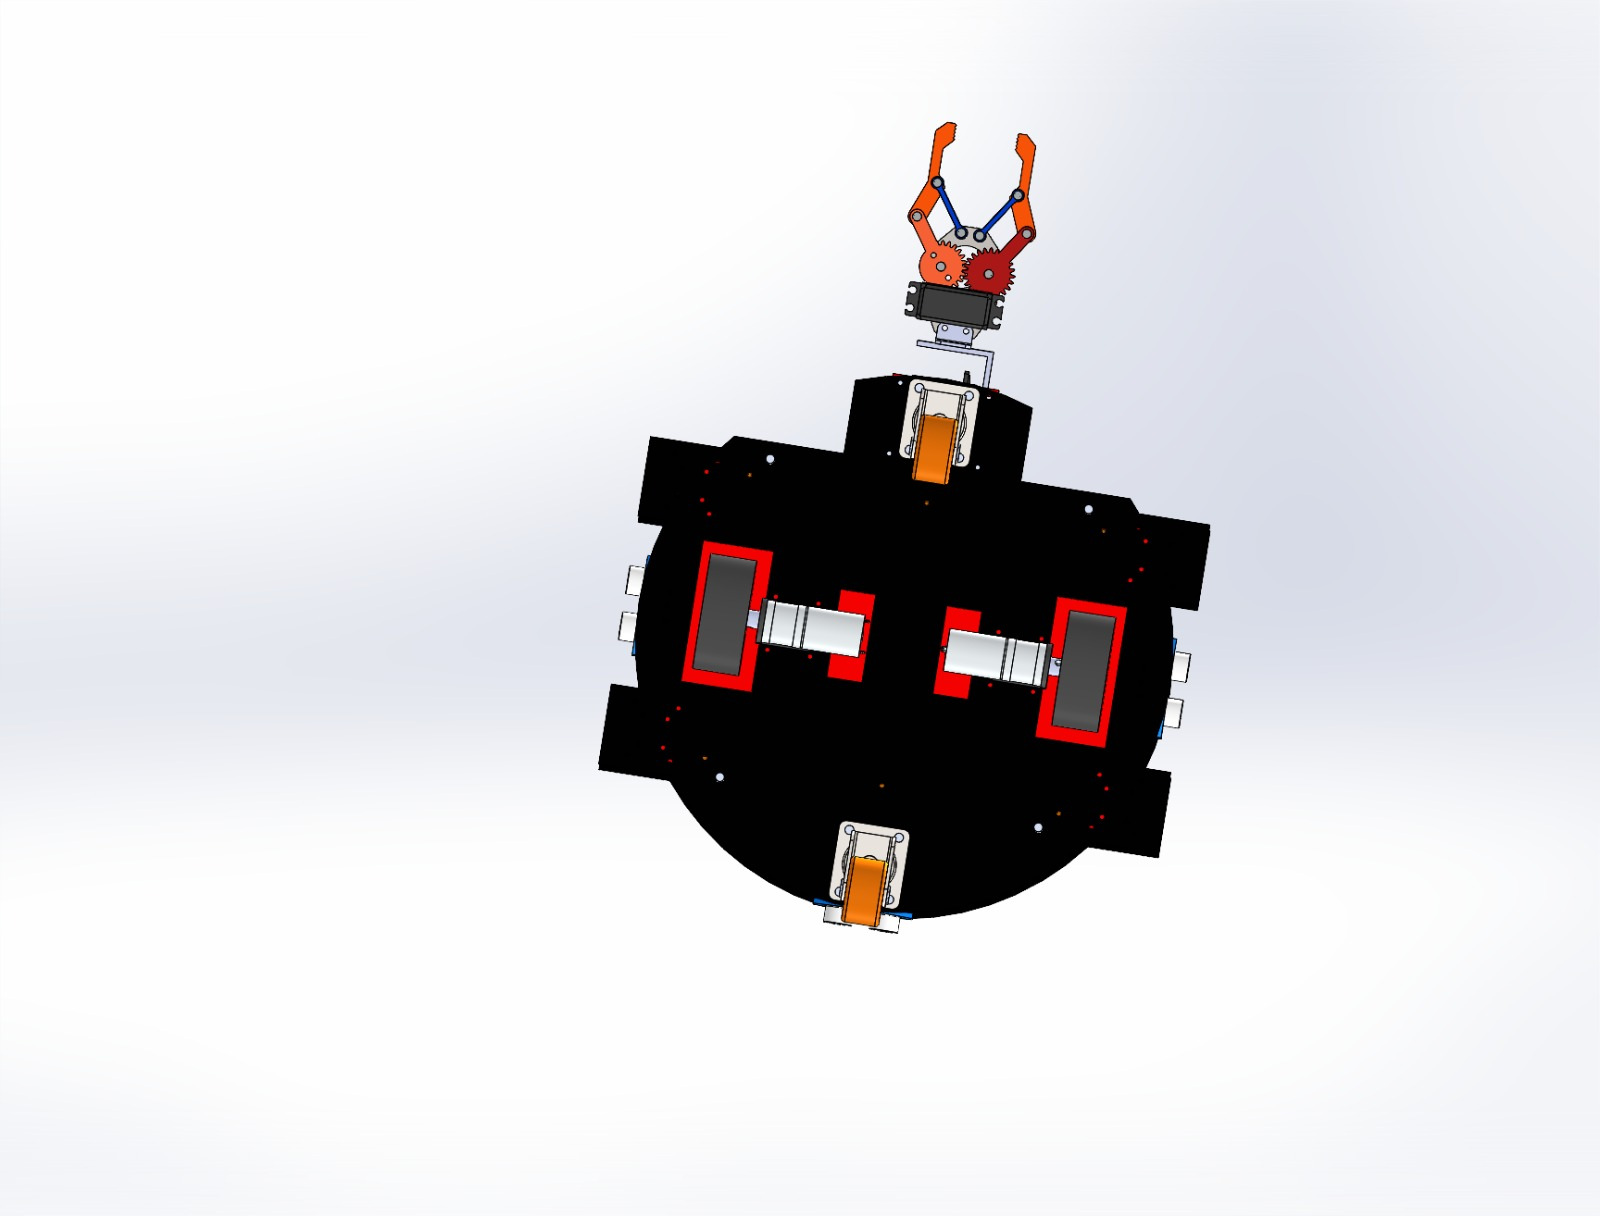
\includegraphics[scale=0.23]{./Figures/Mech/lower.jpeg}
	\caption{Final Design -- Bottom view}
	\label{fig:mech2}
\end{figure}
\newpage
\begin{figure}[h!]
	\centering
	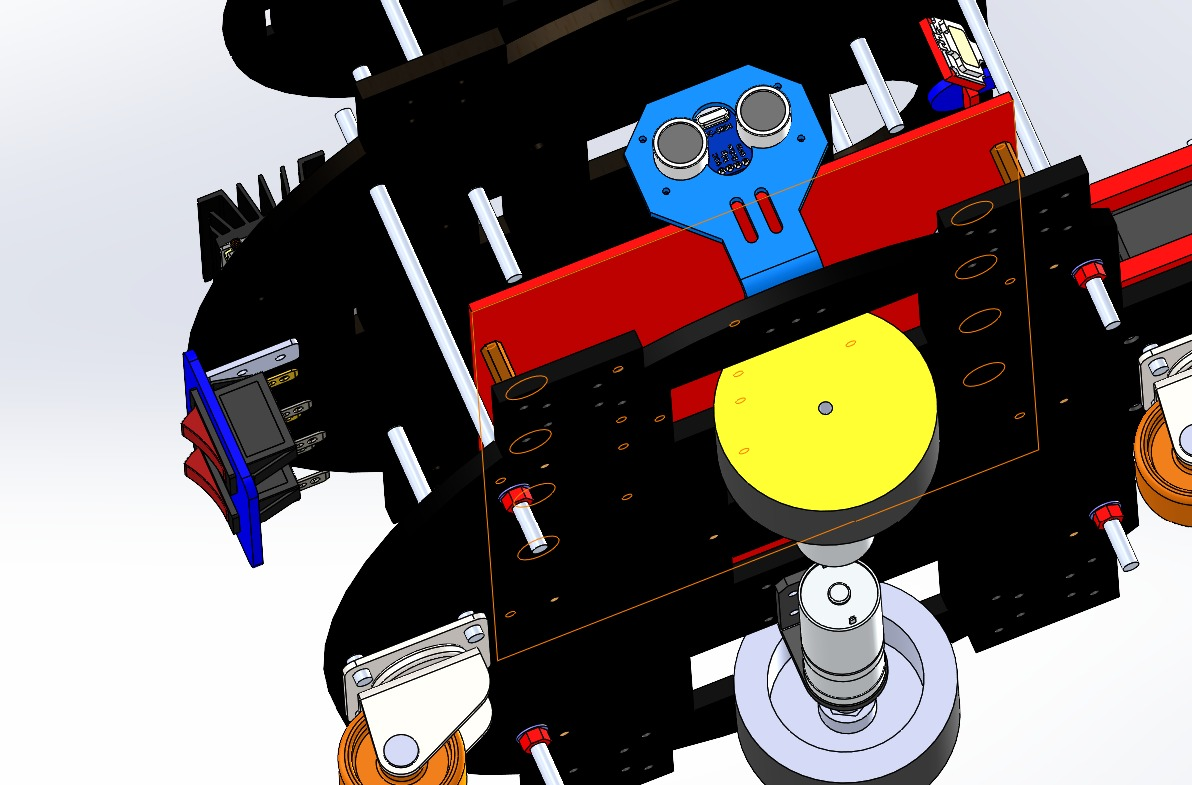
\includegraphics[scale=0.32]{./Figures/Mech/side.jpeg}
	\caption{Final Design -- Side view}
	\label{fig:mech3}
\end{figure}

\begin{figure}[h!]
	\centering
	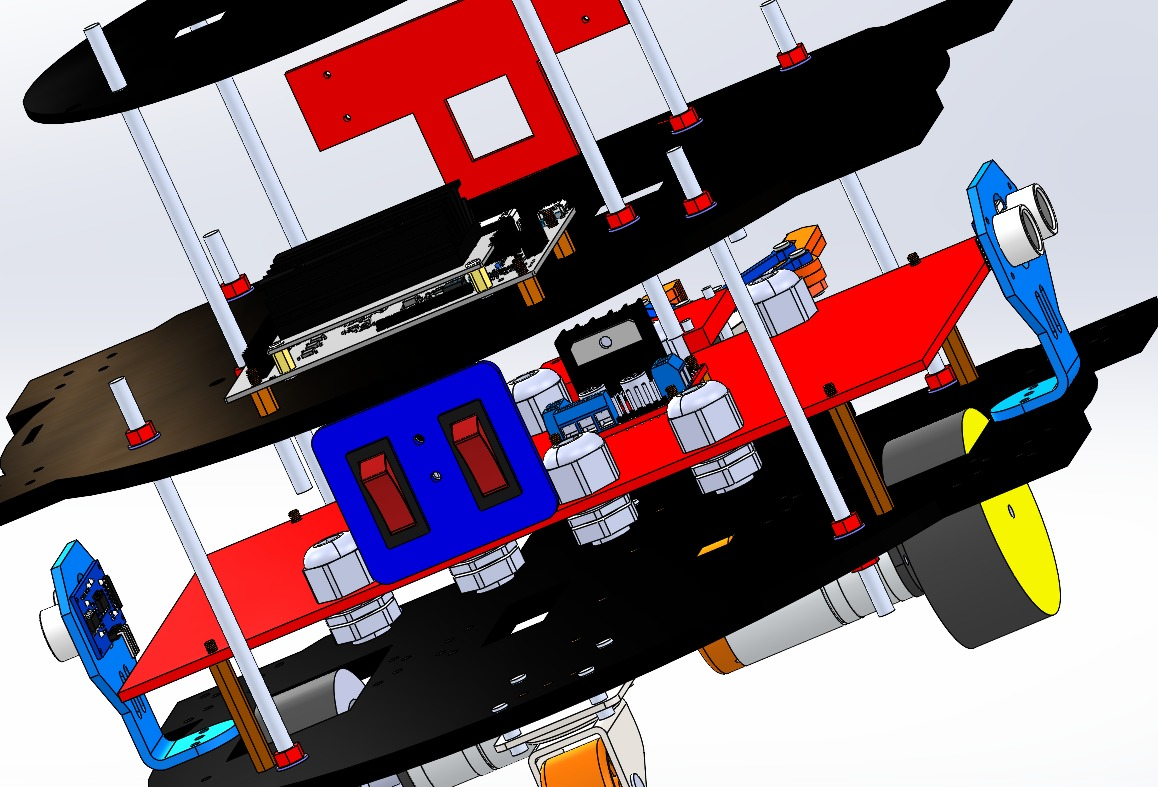
\includegraphics[scale=0.32]{./Figures/Mech/bacc.jpeg}
	\caption{Final Design -- Back view}
	\label{fig:mech4}
\end{figure}
\newpage
% \notrickroll

% \lstinputlisting[language=C, style=CodeStyleC, caption=test code, label=cd:haha, firstline=1, lastline=6]{CodeSnippets/haha.c}
